\chapter{Progettazione e codifica}
\label{cap:progettazione-codifica}

\intro{Breve introduzione al capitolo}\\

\section{Tecnologie e strumenti}
\label{sec:tecnologie-strumenti}

Di seguito viene data una panoramica delle tecnologie e strumenti utilizzati.

\subsection*{Tecnologia 1}
Descrizione Tecnologia 1.

\subsection*{Tecnologia 2}
Descrizione Tecnologia 2

\section{Ciclo di vita del software}
\label{sec:ciclo-vita-software}

\section{Progettazione}
\label{sec:progettazione}
In questo capitolo vengono descritte in dettaglio le dipendenze e i metodi di ciascuna classe presente nell'architettura software utilizzata dal sistema.
Ai fini di una maggior comprensione vengono forniti i diagrammi UML delle classi prodotti durante il periodo di progettazione del software e migliorati durante il corso del progetto.
\subsection{Panoramica generale} %**************************
Lo schema seguente contiene una visione generale dei componenti che costituiscono il sistema omettendone gli aspetti secondari che verranno descritti nelle sezioni dedicate di seguito.
\newpage
\begin{landscape}
\pagestyle{fancy}

\begin{figure}[!h] 
    \centering
    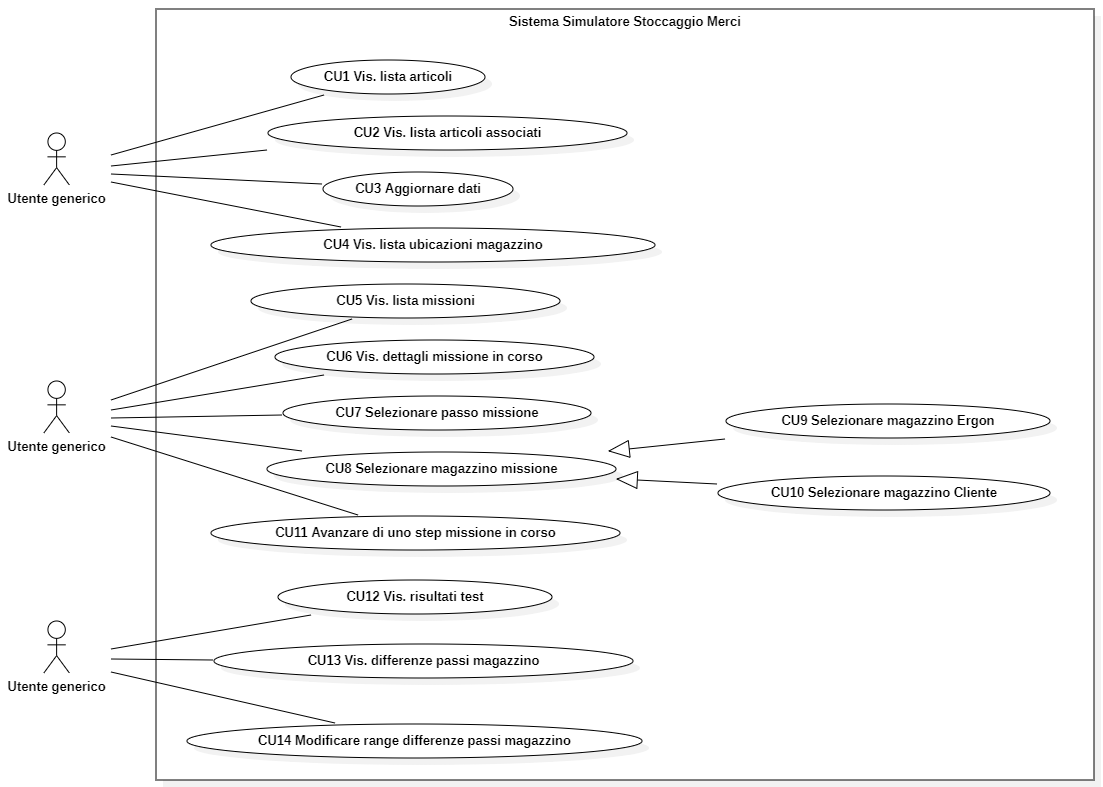
\includegraphics[width=\linewidth, keepaspectratio]{../stage/materiale\_tesi/Materiale\_tesi/Codice/screen\_classi/generale.png} 
    \caption{UML panoramica generale}
\end{figure}  
\end{landscape}
\subsection{Classi modello di business} %**************************
Il modello di business costituisce la logica di business del sistema.
\begin{figure}[!h] 
    \centering 
    \makebox[\textwidth]{
        \includegraphics[width=1.5\columnwidth]{../stage/materiale\_tesi/Materiale\_tesi/Codice/screen\_classi/modello\_business.png} 
        }
        \caption{UML modello di business}
    \end{figure}
\textbf{ModelloArticoli}\\
Classe che contiene il dizionario degli articoli disponibili al sistema e le loro associazioni e un dizionario con i dettagli di interesse di ogni articolo.
\textbf{Dipendenze}:
\begin{itemize}
    \item Articolo(Aggregazione): crea gli articoli che verranno utilizzati dal sistema;\\
    \item ErgdisEntities(Associazione): utilizzato per recuperare dal database gli articoli disponibili che il sistema utilizza.\\
\end{itemize}
\textit{Costruttori}:\\
\begin{itemize}
    \item ModelloArticoli(in ums:List<string>)\\
    Crea un'istanza di ModelloArticoli utilizzando la lista ums parametro formale per reperire dal database gli articoli che hanno unità di misura contenuta nella lista.
    Ars rappresenta il dizionario delle associazioni tra articoli mentre arts\_det contiene le informazioni utili di ogni articolo.
\end{itemize}
\textit{Metodi pubblici}:\\
\begin{itemize}
    \item AggiornaDati(): void \\
    Metodo chiamato quando l'utente interagisce con il sistema per aggiornare i dati da visualizzare, in particolare la lista degli articoli e degli associati di ogni articolo.
    \item GetArts(): Dictionary<string-Dictionary<string-int>> \\
    Ritorna il dizionario delle associazioni articoli.
    \item GetDet(): Dictionary<string-Articolo> \\
    Ritorna il dizionario che contiene i dettagli di ogni articolo.
    \item GetArtsAssoc(in cod\_art:string): Dictionary<string-Dictionary<string-int>> \\
    Ritorna il dizionario degli articoli associati all'articolo con codice articolo uguale al parametro formale cod\_art.
    \item GetDetArt(in cod\_art:string): Articolo. \\
    Ritorna l'articolo con codice articolo specificato da cod\_art parametro formale da cui è possibile ricavare i dettagli dell'articolo.
\end{itemize} 
\textit{Metodi privati}:\\
\begin{itemize}
    \item CreaDizionarioArts(): void \\
    Metodo che crea il dizionario degli articoli associati. Quando viene chiamato il metodo svuota il dizionario corrente e ne crea un altro aggiornato con i dati più recenti 
    interrogando il database.
    \item CreaDizionarioArtsDet(): void \\
    Metodo che crea il dizionario dei dettagli di ogni articolo. Quando viene chiamato il metodo, svuota il dizionario corrente e ne crea un altro aggiornato con i dati più recenti 
    interrogando il database.
\end{itemize} 





\subsection{Classi utili al modello di business} %**************************
Di seguito sono riportate le classi che vengono utilizzate dal modello di business.
\\\\
\begin{figure}[!h] 
    \centering 
    \makebox[\textwidth]{
    \includegraphics[width=1.5\columnwidth]{../stage/materiale\_tesi/Materiale\_tesi/Codice/screen\_classi/utili\_modello\_business.png} 
    }
    \caption{UML classi utili al modello di business}
\end{figure}
\textbf{Magazzino}
\\
Rappresenta un magazzino sul quale può essere eseguita una \gls{simulazione di prelievog} o i
test sul numero di fermate e sulla distanza percorsa per completarla.
Un magazzino contiene gli articoli che vengono disposti nei punti di prelievo a seconda del passo associazione o della disposizione degli articoli presenti all'interno del magazzino cliente.
Un punto di prelievo può contenere un solo articolo.
Tramite il carrello vengono prelevati gli articoli fino al completamento della missione di prelievo.
La posizione del carrello all'interno del magazzino viene indicata dalla posizione in cui si trova la sua ultima sezione che è la sezione ad indice minore rispetto alle posizioni di prelievo.\\\\
\textbf{Dipendenze}:
\begin{itemize}
    \item Carrello (Associazione): utilizzata per svolgere le simulazioni di prelievo;
    \item Articolo (Associazione): utilizzata per inizializzare i punti di prelievo.\\
\end{itemize}
\textbf{I metodi principali della classe sono}:
\\\\
\textit{Costruttori}:
\begin{itemize}
    \item Magazzino(in dim:int, in car:Carrello)\\
    Crea un'istanza di un magazzino con dim punti di prelievo e utilizza il carrello car per scorrere e prelevare gli articoli dai punti di prelievo;\\
    dim: dimensione del magazzino che corrisponde al numero di ubicazioni e quindi di articoli che possono essere stoccati all'interno dei punti di prelievo;\\
    car: carrello utilizzato per scorrere i punti di prelievo e prelevarne gli articoli.\\
\end{itemize}
\textit{Metodi per popolare il magazzino}:
\begin{itemize}
    \item PopolaMagazzino(in articoli:List<Articolo>): void\\
    Inizializza i punti di prelievo con gli elementi del parametro articoli seguendo l'ordine in cui si trovano all'interno della lista;
    \item PopolaMagazzino(in passo:int, in articoli:List<Articolo>, in strut\_associati: Dictionary<string-Dictionary<string-int> >): void\\
    Inizializza i punti di prelievo con gli elementi della lista articoli seguendo il passo fornito e la strut\_associati.\\
    passo: rappresenta il numero di articoli associati da disporre nelle posizioni contigue dei punti di prelievo.\\
    articoli: rappresenta gli articoli da utilizzare per inizializzare i punti di prelievo.\\
    strut\_associati: dizionario che ha come chiavi i codici univoci degli articoli presenti nella lista articoli e come valori i dizionari aventi come chiavi 
    i codici articoli che sono associati all'articolo chiave e come valori il numero di volte che l'associato compare all'interno di un ordine cliente assieme all'articolo chiave.\\
\end{itemize}
\textit{Metodi per la gestione del carrello}:
\begin{itemize}
    \item GetPosCarrello(): int\\
    Ritorna la posizione della sezione ad indice minore del carrello;
    \item GetPuntiPrelievoCarrello(): Array<Articolo>\\
    Ritorna gli articoli che corrispondono al range di prelievo del carrello quindi gli articoli che sono prelevabili dalla posizione in cui si trova il carrello;
    \item CaricaCoperturaCarrello(): void\\
    Carica nelle corrispettive sezioni del carrello gli articoli che sono target nella missione in corso e che sono all'interno della copertura del carrello;
    \item GetCoperturaCarrello(): List<int>\\
    Ritorna la lista di indici delle posizioni di prelievo all'interno della copertura del carrello;
    \item MuoviCodaCarrello(in pos:int): void\\
    Sposta la coda del carrello alla posizione indicata dal parametro pos.\\
\end{itemize}
\textit{Metodi per l'esecuzione dei test}:
\begin{itemize}
    \item TestValutazioneFermate(): int\\
    Ritorna il numero di fermate impiegate dal carrello per completare la missione di prelievo che gli è stata assegnata;
    \item TestValutazioneDistanza(): int\\
    Ritorna la distanza percorsa dal carrello per completare la missione di prelievo che gli è stata assegnata.\\
\end{itemize}
\textit{Metodi privati di utilità}:
\begin{itemize}
    \item ControlloArticoliMissionePresenti(): bool\\
    Ritorna true se tutti gli articoli coinvolti nella missione assegnata al carrello sono presenti all'interno dei punti di prelievo altrimenti false.
    Nel caso ritorni true viene garantito che la missione assegnata al carrello possa essere completata con successo;
    \item GetIndiceProssimoArtInMissioni(): int\\
    Ritorna l'indice del prossimo articolo da prelevare per la missione assegnata al carrello;
    \item GetMigliorAssociato(in cod:string, in strut:Dictionary<string-int>): string\\
    Metodo di utilità utilizzato principalmente durante il popolamento del magazzino.\\
\end{itemize}       
\textbf{Carrello}\\
Rappresenta il carrello fisico che si muove all'interno di un magazzino per prelevare gli articoli dai punti di prelievo.
Il numero di posti corrisponde al numero di sezioni e ogni sezione può contenere gli articoli riguardanti un solo ordine cliente.
Dato che l'obiettivo del progetto è focalizzato sullo stoccaggio della merce è stato assunto che tutti gli articoli appartenenti ad un ordine 
da completare possano essere collocati nelle sezioni relative senza tenere conto di vincoli fisici.
La classe presenta due contatori che tengono conto della distanza percorsa (espressa in punti di prelievo visitati) e il numero di fermate effettuate
(il punto da cui parte il carrello non viene contata).\\
\textbf{Dipendenze}:
\begin{itemize}
    \item Missione (Associazione): corrisponde alla missione assegnata al carrello durante la simulazione di prelievo.\\
\end{itemize}
\textbf{I metodi principali della classe sono}:\\
\textit{Costruttori}:\\
\begin{itemize}
    \item Carrello(in n\_posti:int, in mis:Missione):\\
    Crea un'istanza di un carrello con n\_posti e gli assegna la missione mis.\\
\end{itemize}
\textit{Metodi pubblici}:\\
\begin{itemize}
    \item Carica(in cod\_art:string, in pos\_prelievo:int): void\\
    Imposta la posizione di prelievo del target missione corrispondente al cod\_art alla pos\_prelievo;
    \item Pieno(): bool\\
    Ritorna true se tutte le sezioni del carrello sono occupate da almeno un articolo ovvero quando il numero di posti occupati 
    corrisponde al numero di posti totale, altrimenti false;
    \item Svuota(): void\\
    Imposta il numero di posti occupati a zero;
    \item Reset(): void\\  
    Imposta il numero di posti occupati,il numero di fermate effettuate e la distanza percorsa a zero; inoltre ripristina la missione che gli è stata assegnata.\\
\end{itemize} 
\textbf{Missione}\\
Rappresenta la missione assegnata al carrello che deve essere completata durante la simulazione di prelievo prelevando i target missione dai punti di prelievo.\\
\textbf{Dipendenze}:
\begin{itemize}
    \item Target (Associazione): un target corrisponde ad un articolo da prelevare per completare la missione.
\end{itemize}
\textbf{I metodi principali della classe sono}:\\
\textit{Costruttori}:\\
\begin{itemize}
    \item Missione(in targets:List<Target>)\\
    Crea un'istanza di una missione con lista target uguale a targets parametro formale;
    \item Missione(in missione:Missione)\\
    Costruttore di copia profonda.\\
\end{itemize}
\textit{Metodi pubblici}:\\
\begin{itemize}
    \item SetPosPrelievoTarget(in cod\_art:string, in pos\_prelievo:int): void\\
    Imposta la posizione di prelievo a pos\_prelievo dell'articolo con codice articolo cod\_art nella lista dei target;
    \item MissioneCompletata(): bool\\
    Ritorna true se tutti i target missione all'interno della lista target hanno una posizione di prelievo diversa da -1 altrimenti false.
    Un target con posizione di prelievo diversa da -1 è stato prelevato dalla posizione di prelievo indicata dal valore impostato.
    \item Ripristina(): void\\
    Imposta tutte le posizioni di prelievo dei target missione a -1.
    \item GetTargets(): List<Target>\\
    Ritorna la lista dei target missione.\\
\end{itemize} 
\textbf{Target}\\
Rappresenta un articolo da prelevare per completare una missione di prelievo.
Un target viene identificato dal codice articolo da prelevare, dall'ordine a cui appartiene (numero ordine e anno ordine) e dalla posizione
di prelievo da cui è stato prelevato (se non ancora prelevato la posizione di prelievo ha valore -1)\\
\textbf{I metodi principali della classe sono}:\\
\textit{Costruttori}:\\
\begin{itemize}
    \item Target(in cod\_art:string, in nr\_ord:int, in anno\_ord:int)\\
    Crea un'istanza di un target assegnando ai campi dati corrispondenti i parametri formali;
    \item Target(in target:Target)\\
    Costruttore di copia profonda.\\
\end{itemize}
\textit{Metodi pubblici}:\\
I metodi che offre la classe sono i metodi getter e setter per ricavare o impostare i valori dei campi dati.\\
\textbf{ErgdisEntities}\\
Classe che contiene i riferimenti agli oggetti che rappresentano le entità di interesse fornite dal DB.
Viene utilizzata per interfacciarsi al DB.
Tutte le dipendenze di cui necessita la classe vengono generate automaticamente da Entity Framework. Per aggiungere un'entità basta aggiornare
la classe utilizzando le funzionalità offerte dall'IDE di sviluppo tramite interfaccia grafica.
\textbf{Dipendenze}:
\begin{itemize}
    \item DettagliOrdiniCliente (Associazione): \\
    Classe che rappresenta i dati presenti a database nella tabella DettagliOrdiniCliente.\\
    La tabella è strutturata in modo che ogni record contiene le informazioni per un articolo presente in un ordine cliente in modo da
    fornirne il codice, il numero dell'ordine e l'anno dell'ordine.
    \item AnagraficaArticoli (Associazione): \\
    Classe che rappresenta i dati presenti a database nella tabella AnagraficaArticoli.\\
    La tabella è strutturata in modo che ogni record contiene le informazioni utili a reperire le informazioni relative ad ogni singolo articolo (codice articolo,descrizione,unità di misura ecc.).
    \item AnagraficaArticoliMagazzinoCliente (Associazione): \\
    Classe che rappresenta i dati presenti a database nella tabella AnagraficaArticoliMagazzinoCliente.\\
    La tabella è strutturata in modo che ogni record contiene le informazioni utili a reperire le informazioni relative ad ogni singolo articolo in relazione con il magazzino cliente.
    Ad esempio un dato utile da ricavare da questa tabella potrebbe essere il codice del deposito in cui è stoccato l'articolo.
    \item FrequenzeArticoli (Associazione): classe che rappresenta i dati presenti a database nella tabella FrequenzaArticoli.
    Tiene traccia dei codici articoli e delle frequenze di vendita di ciascuno ovvero quante volte gli articoli compaiono all'interno degli 
    ordini cliente. La classe permette di velocizzare i tempi di caricamento a runtime dell'applicazione in quanto avendo salvato a database
    le frequenze di vendita non è necessario ricalcolarle ogni volta che si avvia l'applicazione. Questo ha portato ad un aumento evidente delle 
    performance durante il caricamento iniziale della finestra principale;\\
    \item AssociazioniArticoli (Associazione): classe che rappresenta i dati presenti a database nella tabella AssociazioniArticoli.
    Presenta i campi cod\_art e cod\_art\_assoc e con il campo freq\_assoc viene memorizzato il numero di volte che il primo articolo è
    presente all'interno degli ordini clienti assieme al secondo articolo.
    Anche questa classe permette di velocizzare i tempi di caricamento evitando di ricalcolare ad ogni esecuzione le frequenze di associazione
    tra gli articoli.\\
    \item Database (Associazione): classe utilizzata per interagire con il database.\\
\end{itemize}

\textbf{ComparatoreDiffPassiMagazzini}\\
Classe utilizzata per confrontare i risultati dei test eseguiti tra configurazioni diverse di magazzini.
\textbf{Dipendenze}:
\begin{itemize}
    \item Magazzino (Associazione): rappresenta i magazzini da confrontare.\\
\end{itemize}
\textbf{I metodi principali della classe sono}:\\
\textit{Costruttori}:\\
\begin{itemize}
    \item ComparatoreDiffPassiMagazzini(in magazzino1:Magazzino, in magazzino2:Magazzino, in inizio\_range:int, in fine\_range:int):\\
    Crea un'istanza di ComparatoreDiffPassiMagazzini con magazzino1 e magazzino2 da confrontare ed imposta il range di ubicazioni all'interno dei magazzini da confrontare secondo i parametri inizio\_range e fine\_range.\\ 
\end{itemize}
\textit{Metodi pubblici}:\\
\begin{itemize}
    \item GetDiffPosizioni(): int \\
    Ritorna il numero di ubicazioni che non contengono gli stessi articoli agli indici corrispondenti nei punti prelievo.
    Questo metodo viene utilizzato per confrontare configurazioni di magazzino che hanno passi associazione diversi in modo da poter capire quanti articoli non si trovano nelle stesse posizioni
    rispetto a passi associazioni diversi;\\
    \item GetDiffArticoli(): int \\
    Ritorna il numero di articoli che non sono presenti nel primo magazzino e sono presenti all'interno del secondo magazzino.
    Questo metodo viene utilizzato per confrontare configurazioni di magazzino che hanno passi diversi in modo da poter capire quanti articoli non si trovano all'interno del range in passi associazioni diversi;\\
    \item GetCodArtRange(): List<string> \\
    Ritorna i codici degli articoli che si trovano all'interno del range di confronto (tra inizio\_range e fine\_range compresi).\\
\end{itemize} 
\subsection{Classi utili alle viste}
Di seguito sono riportate le classi che vengono utilizzate dalle viste per rappresentare le informazioni di interesse per l'utente.
\\\\
 
\textbf{ResocontoTest}\\
Classe astratta che rappresenta un set di test eseguiti e ne raccoglie i risultati ottenuti ed altre informazioni tra le quali il nome e una descrizione testuale dei test eseguiti.
\textbf{Estesa da}:
\begin{itemize}
    \item ResocontoTestCliente: raccoglie i test eseguiti sul magazzino cliente senza passo associazioni;
    \item ResocontoTestErgon: raccoglie i risultati dei test sul magazzino Ergon con passo associazioni.\\
\end{itemize}
\textit{Costruttori}:\\
\begin{itemize}
    \item ResocontoTest(): utilizzato dalle sottoclassi per inizializzarne i campi dati.\\
\end{itemize}
\textit{Metodi pubblici}:\\
I metodi messi a disposizione sono i getter e setter per il nome e la descrizione dei test presenti all'interno del resoconto.\\
\textbf{ResocontoTestCliente}\\
Classe che contiene i test effettuati sul magazzino cliente e ne contiene le informazioni di interesse.\\
\textbf{Estende}:\\
ResocontoTest\\
\textbf{Dipendenze}:
\begin{itemize}
    \item RisultatoTestCliente (Associazione): risultato di un test effettuato sul magazzino cliente.\\
\end{itemize}
\textit{Costruttori}:\\
\begin{itemize}
    \item ResocontoTestCliente(in risultati:List<RisultatoTestCliente>):\\
    Crea un'istanza di ResocontoTestCliente che contiene i risultati dei test effettuati sul magazzino cliente.\\
\end{itemize}
\textit{Metodi pubblici}:\\
I metodi pubblici della classe sono i getter e i setter per ricavare i valori dei campi dati.\\
\textbf{ResocontoTestErgon}\\
Classe che contiene i test effettuati sul magazzino Ergon e ne contiene le informazioni di interesse.\\
\textbf{Dipendenze}:
\begin{itemize}
    \item RisultatoTestErgon (Associazione): risultato di un test effettuato sul magazzino Ergon quindi con passo associazioni articoli.\\
\end{itemize}
\textit{Costruttori}:\\
\begin{itemize}
    \item ResocontoTestErgon(in risultati:List<RisultatoTestErgon>):\\
    Crea un'istanza di ResocontoTestErgon che contiene i risultati dei test effettuati sul magazzino Ergon.
\end{itemize}
\textit{Metodi pubblici}:\\
\begin{itemize}
    \item I metodi pubblici della classe sono i getter e i setter per ricavare i valori dei campi dati.\\
\end{itemize} 
\textbf{RisultatoTestCliente}\\
Un RisultatoTestCliente rappresenta il risultato di un test avvenuto sul magazzino cliente senza passo associazioni utilizzando un carrello  per effettuare i prelievi 
dalle posizioni di magazzino.
Il risultato ha come campi dati il nome del cliente e il codice del deposito su cui avviene il test.\\
\textbf{Estende}:\\
RisultatoTestCarrello\\
\textbf{Implementa}:\\
RisultatoTestCarrello\\
\textit{Costruttori}:\\
\begin{itemize}
    \item RisultatoTestCliente(in nome\_cliente:string, in cod\_dep:string, in dimCarrello:int).\\
    Crea un'istanza di RisultatoTestCliente ed imposta i campi dati con i parametri passati come parametri formali.\\
\end{itemize}
\textit{Metodi pubblici}:\\
\begin{itemize}
    \item I metodi pubblici della classe sono i getter e i setter per ricavare i valori dei campi dati.\\
\end{itemize} 
\textbf{RisultatoTestDistanzaCliente}\\
Rappresenta un risultato di un test distanza effettuato sul magazzino cliente e ne memorizza la distanza percorsa dal carrello per completare il test.\\
\textbf{Estende}:\\
RisultatoTestCliente\\
\textbf{Implementa}:\\
RisultatoTestDistanza\\
\textit{Costruttori}:\\
\begin{itemize}
    \item RisultatoTestDistanzaCliente(in nome\_cliente:string, in cod\_dep:string, in dimCarrello:int).\\
    Crea un'istanza di RisultatoTestDistanzaCliente ed imposta i campi dati con i parametri passati come parametri formali.\\
\end{itemize}
\textit{Metodi pubblici}:\\
\begin{itemize}
    \item I metodi pubblici della classe sono i getter e i setter per ricavare i valori dei campi dati.\\
\end{itemize} 

\textbf{RisultatoTestFermateCliente}\\
Rappresenta un risultato di un test fermate effettuato sul magazzino cliente e ne memorizza il numero di fermate impiegate dal carrello per completare il test.\\
\textbf{Estende}:\\
RisultatoTestCliente\\
\textbf{Implementa}:\\
RisultatoTestFermate\\
\textit{Costruttori}:\\
\begin{itemize}
    \item RisultatoTestFermateCliente(in nome\_cliente:string, in cod\_dep:string, in dimCarrello:int).\\
    Crea un'istanza di RisultatoTestFermateCliente ed imposta i campi dati con i parametri passati come parametri formali.\\
\end{itemize}
\textit{Metodi pubblici}:\\
\begin{itemize}
    \item I metodi pubblici della classe sono i getter e i setter per ricavare i valori dei campi dati.\\
\end{itemize}
\textbf{RisultatoTestCarrello}\\
Rappresenta un risultato di un test effettuato utilizzando un carrello per il prelievo degli articoli dal magazzino.
\textbf{Classe base di}:
\begin{itemize}
    \item RisultatoTestCliente;
    \item RisultatoTestErgon.\\
\end{itemize}
\textit{Costruttori}:\\
\begin{itemize}
    \item RisultatoTestCarrello(in int dim\_carrello).\\
\end{itemize}
\textit{Metodi pubblici}:\\
\begin{itemize}
    \item GetDimCarrello(): int\\
    Ritorna la dimensione del carrello con cui è stato effettuato il test.\\
\end{itemize} 

\subsection{Forms e componenti utili} %**************************
Di seguito sono riportate le classi che partecipano al funzionamento delle finestre dell'applicazione.

\textbf{Form1}\\
Form1 utilizza i componenti DevExpress per fornire all'utente la lista degli articoli disponibili 
e i loro associati oltre alle funzionalità di avvio simulazione e di aggiornamento dei dati utilizzati dal sistema.
\textbf{Dipendenze}:
\begin{itemize}
    \item Controller1 (Associazione): utilizza il controller che ne gestisce la logica per recuperare le informazioini da visualizzare dal ModelloArticoli.\\
\end{itemize}
\textit{Costruttori}:\\
\begin{itemize}
    \item Form1(in articoli:List<Articolo>, in associati:List<ArticoloAssociato>)\\
    Crea un'istanza di Form1 utilizzando le liste passate come parametri per visualizzare gli articoli presenti e 
    gli articoli associati dell'articolo più frequente nelle relative grid di visualizzazione.
\end{itemize}
\textit{Metodi privati}:\\
\begin{itemize}
    \item AggiornaGridAssociati(in sender:object, in args\_event:RowCellClickEventArgs): void\\
    Aggionrna i dati della grid relativa agli articoli associati per mostrare all'utente 
    gli articoli associati dell'articolo selezionato;
    \item AggiornaDati(in sender:object, in args\_event:ItemClickEventArgs): void \\
    Aggiorna i dati che il sistema utilizza quando l'utente accede alla funzionalità aggiornamento dati;
    \item AvviaSimulazione(in sender:object, in args\_event:EventArgs): void \\
    Avvia la simulazione di prelievo aprendo Form2 che si occupa della gestione della simulazione. 
\end{itemize} 

\textbf{Controller1}\\
Controller1 gestisce la logica dell'applicazione per Form1 facendo comunicare il componente con il modello articoli.
Inoltre ha lo scopo di creare il controller che gestisce la simulazione missione quando l'utente accede alla relativa funzionalità.
\textbf{Dipendenze}:
\begin{itemize}
    \item ModelloArticoli(Associazione): interroga il modello articoli per fornire alla Form1 gli articoli da visualizzare\\
    \item Form1(Composizione): gestisce l'intero ciclo di vita di Form1.
    \item ControllerSimulazione(Dipendenza semplice: create): crea l'istanza di ControllerSimulazione.
\end{itemize}
\textit{Costruttori}:\\
\begin{itemize}
    \item Controller1(in AppInfo info)\\
    Crea un'istanza di Controller1 utilizzando le info passate come parametro formale per stabilire una connessione con il database.
    Le info fanno parte della classe statica Program che è un singleton per il sistema.
\end{itemize}
\textit{Metodi pubblici}:\\
\begin{itemize}
    \item AggiornaGridArticoli(in cod\_um:string): void\\
    Aggiorna la grid articoli prensente in Form1 con gli articoli presenti nel modello che hanno come codice unità di misura quello passato come parametro formale.
    \item AggiornaGridAssociati(in cod\_art:string): void
    Aggiorna la grid articoli associati con gli articoli che sono associati all'articolo con codice articolo passato come parametro formale.
    \item AggiornaDB(): void
    Aggiorna i dati presenti nel modello  articoli con i dati presenti a database.
    Questa operazione viene svolta solo su richiesta dell'utente in quanto risulta essere molto dispendiosa nel calcolo delle associazioni.
    \item AvviaSimulazione(in modello\_articoli:ModelloArticoli, in date\_ordini:List<DateTime>, in ums:List<string>): void \\
    Metodo che crea un'istanza di ControllerSimulazione che gestisce la logica dell'applicazione riguardante una simulazione di prelievo.
    Viene invocato quando l'utente interagisce con il sistema per avviare una simulazione di prelievo che utilizza i dati presenti nel modello articoli
    per inizializzare la simulazione.
\end{itemize} 
\textit{Metodi privati}:\\
\begin{itemize}
    \item RimuoviPrimoLivelloUm(in arts:Dictionary<string-Dictionary<string-int>>, in lista\_um:List<string>): Dictionary<string-Dictionary<string-int>>
    Metodo che dato un dizionario arts mantiene le chiavi (codici articoli) i cui articoli hanno unità di misura presente nella lista\_um parametro formale rimuovendo gli altri.
    Questo può essere utile per visualizzare in grid articoli solo gli articoli di interesse filtrando quelli che non rispettano le unità di misura desiderate. 
    \item RimuoviSecondoLivelloUm(in arts:Dictionary<string-int>, in lista\_um:List<string>): Dictionary<string-int>
    Metodo che dato un dizionario che rappresenta gli articoli associati ad un articolo ne rimuove quelli che non hanno unità di misura presente all'interno di lista\_um
    parametro formale.
\end{itemize}  
\textbf{FormSimulazione}\\
FormSimulazione è la classe utilizzata per creare la finestra per la visualizzazione di una simulazione di prelievo.
Viene mostrata quando l'utente avvia una simulazione di prelievo interagendo con il sistema.
\textbf{Dipendenze}:
\begin{itemize}
    \item SezioneCarrello(Composizione): crea le istanze delle sezioni del carrello che servono a contenere i dati per la visualizzazione del contenuto del carrello all'interno delle CardView relative a
    ciascuna sezione;\\
    \item ControllerSimulazione(Associazione): viene utilizzato per aggiornare i dati relativi alla simulazione di prelievo in corso quando l'utente interagisce con il sistema.
\end{itemize}
\textit{Costruttori}:\\
\begin{itemize}
    \item FormSimulazione(in arts\_magazzino:List<Articolo>, in magazzino\_selezionato:string, in passo:int, in magazzini\_disponibili:List<string>)\\
    Crea un'istanza di FormSimulazione che ha lo scopo di rappresentare i dati relativi alla rimulazione di prelievo in corso utilizzando i componenti DevExpres.
    Il costruttore utilizza arts\_magazzino per inizializzare le CardView che rendono disponibile all'utente la lista degli articoli presenti nel magazzino utilizzato durante la simulazione;
    utilizza gli altri parametri per inizializzare i componenti utili all'utente per selezionare altre modalità di simulazione per gli ordini previsti dalla simulazione in corso (ad esempio per avviare 
    una simulazione con passo differente o su un altro magazzino).
\end{itemize}
\textit{Metodi pubblici}:\\
\begin{itemize}
    \item CreaNuovaMissione(in dim\_carrello:int): void\\
    Metodo chiamato quando viene avviata una nuova simulazione di prelievo. Il metodo utilizza gli articoli presenti nel magazzino della simulazione precedente per avviare la nuova simulazione e utilizza 
    la dim\_carrello per inizializzare le sezioni del carrello visualizzate allo stato vuoto (in seguito verranno create nuove sezioni contenenti gli articoli prelevati ad ogni step missione);
    \item AvanzaMissione(in articoli\_prelevati:List<Articolo>, in missione\_terminata:bool, in missioni\_terminate:bool): void\\
    Avanza di uno step la missione in corso aggiornando le CardView che rappresentano lo stato del carrello allo step successivo.
    Il metodo dispone gli oggetti prelevati appartenenti allo stesso ordine nella stessa sezione del carrello degli altri articoli dello stesso ordine, altrimenti un articolo prelevato occuperà
    una nuova sezione del carrello. Il corretto riempimento delle sezioni del carrello viene garantito dal ControllerSimulazione che ha il compito di garantire che la missione di prelievo 
    sia completabile utilizzando il carrello fornito dalla vista (un carrello con un numero di sezioni inferiore al numero di ordini da prelevare non sarebbe in grado di contenere tutti gli ordini previsti dalla simulazione).
    Se la missione di prelievo risulta completata e sono presenti altre missioni prima di completare la simulazione viene creata una nuova riga di CardView per rappresentare il carrello allo stato 
    vuoto per la missione successiva.
    \item VediStatistiche(): void\\
    Metodo invocato quando l'utente interagisce con il sistema per visualizzare le statistiche riguardanti tutte le possibili simulazioni di prelievo disponibili per il magazzino cliente e per tutti i passi magazzino Ergon.
    Il metodo interagisce con ControllerSimulazione che apre la finestra di visualizzazione statistiche.
    \item CambiaPasso(): void\\
    Metodo chiamato quando l'utente interagisce con il sistema per avviare una nuova simulazione di prelievo che utillizza un passo associazione articoli diverso dalla missione di prelievo corrente.
    Viene ripristinata la missione allo step iniziale e vengono aggiornati gli articoli presenti a magazzino secondo il passo associazione selezionato e le sezioni del carrello allo stato vuoto.
    \item CambiaMagazzino(): void\\
    Metodo chiamato quando l'utente interagisce con il sistema per avviare una nuova simulazione di prelievo che utillizza un magazzino diverso dalla missione di prelievo corrente.
    Viene ripristinata la missione allo step iniziale e vengono aggiornati gli articoli presenti a magazzino secondo il magazzino e passo associazione selezionato e le sezioni del carrello allo stato vuoto.
    \item AggiornaSezioniCarrello(in articoli\_prelevati:List<Articolo>): void\\
    Metodo che aggiorna le sezioni del carrello utilizzando gli articoli prelevati allo step successivo. 
\end{itemize} 
\textit{Metodi privati}:\\
\begin{itemize}
    \item AggiornaSezioniCarrello(in articoli\_prelevati:List<Articolo>): void\\
    Metodo che aggiorna le sezioni del carrello utilizzando gli articoli prelevati allo step successivo. 
\end{itemize}

\textbf{ControllerSimulazione}\\
Classe che gestisce la simulazione di prelievo avviata dall'utente. Ad ogni interazione comunica con il modello per l'avanzamento o la creazione di una simulazione di prelievo.
\textbf{Dipendenze}:
\begin{itemize}
    \item Simulazione(Aggregazione): modello logico per la simulazione di prelievo gestita dal controller;\\
    \item ControllerTest(Dipendenza semplice: create): crea l'istanza di ControllerTest quando l'utente interagisce con il sistema per visualizzare le statistiche relative 
    alle simulazioni di prelievo disponibili sugli ordini previsti dalla simulazione in corso.
    \item ModelloArticoli(Dipendenza semplice: use): utilizzato per creare un'istanza di Simulazione.
\end{itemize}
\textit{Costruttori}:\\
\begin{itemize}
    \item ControllerSimulazione(in arts:ModelloArticoli, in date\_ordini:List<DateTime>, in ums:List<string>).\\
    Crea un'istanza di ControllerSimulazione che utilizza i parametri formali per creare il modello della simulazione di prelievo.
    Il modello creato per la simulazione utilizzerà solo gli articoli con unità di misura presente nella lista ums parametro formale e ricaverà dal database gli ordini cliente 
    soddisfatti nelle date presesnti in date\_ordini (questo avviene per limitare la simulazione agli ordini soddisfatti in un arco temporale definito e non su tutto lo storico ordini).
\end{itemize}
\textit{Metodi pubblici}:\\
\begin{itemize}
    \item CambiaPassoMissione(in nuovo\_passo:int): void.\\
    Ripristina il modello e la vista secondo il passo simulazione selezionato dall'utente.
    \item CambiaMagazzinoMissione(in ind\_magazzino:int): void \\
    Ripristina il modello e la vista secondo il magazzino selezionato dall'utente.
    \item VediStatistiche(): void \\
    Crea un'istanza di ControllerTest che gestirà la finestra di visualizzazione statistiche.
    Il metodo passa al ControllerTest il ModelloMagazzini che verrà utilizzato per eseguire i test su tutte le configurazioni disponibili e visualizzarne i risultati.
    \item GetModelloMagazzini(): ModelloMagazzini \\
    Ritorna il ModelloMagazzini utilizzato dalla simulazione in corso.
\end{itemize} 
\textbf{Simulazione}\\
Modello logico per una simulazione di prelievo. Tiene conto delle missioni eseguite per completare la simulazione e dell'ordine con cui gli articoli vengono prelevati dal magazzino.
\textbf{Dipendenze}:
\begin{itemize}
    \item Target(Associazione): Utilizza i target missione passati dal client per prelevare gli articoli dal magazzino e per memorizzare le posizioni di prelievo di tali articoli\\
    \item ModelloMagazzini(Aggregazione): Crea il ModelloMagazzini che gestisce le configurazioni di magazzino disponibili.\\
    \item Articolo(Associazione): utilizza gli articoli restituiti dal ModelloMagazzini per memorizzare gl articoli prelevati nello step missione.\\
    \item ModelloArticoli(Dipendenza semplice: use): utilizzato per creare il ModelloMagazzini.
    \end{itemize}
\textit{Costruttori}:\\
\begin{itemize}
    \item Simulazione(in arts:ModelloArticoli,in date\_ordini:List<DateTime>, in ums:List<string>).\\
    Crea un'istanza di Simulazione utilizzando date\_ordini e ums per prelevare dal database gli articoli da prelevare dalla configurazione di magazzino selezionata.
    Utilizza arts per creare il ModelloMagazzini che verrà utilizzato per ricavare la configurazione di magazzino su cui avviare la simulazione.
\end{itemize}
\textit{Metodi pubblici}:\\
\begin{itemize}
    \item AvanzaStepMissione(): int \\
    Avanza di uno step la missione in corso e ritorna lo step aggiornato. Avanzare di uno step significa prelevare dal magazzino selezionato gli articoli dello step successivo 
    e aggiornare le posizioni di prelievo dei relativi target missione. Inoltre vengono incrementate il numero di fermate effettuate e aggiornata la distanza percorsa.
    Articoli prelevati contiene gli articoli prelevati durante lo step in corso;
    \item CambiaPassoMagazzino(in nuovo\_passo:int): void \\
    Metodo che cambia il passo della simulazione ripristinando la simulazione allo stato iniziale;
    Per cambiare il passo simulazione viene reperita la nuova configurazione di magazzino dal ModelloMagazzini che contiene tutte le configurazioni di magazzino disponibili.
    \item ResetSimulazione(): void \\
    Ripristina la simulazione allo stato iniziale;
    \item GetPuntiPrelievo(): Array<Articolo> \\
    Interroga il Modello magazzini per ricavare la disposizione degli articoli del magazzino selezionato ovvero il magazzino sul quale sta avvenendo la simulazione di prelievo.
    \item GetNumeroMissione(): int \\
    Ritorna il numero della missione in corso;
    Ritorna il passo associazione articoli della simulazione in corso;
    \item GetFermate(): int \\
    Ritorna il numero di fermate attuali della simulazione in corso;
    \item GetDistanza(): int \\
    Ritorna la distanza percorsa attuale della simulazione in corso;
    \item GetArticoliPrelevatiStep(): List<Articolo> \\
    Ritorna la lista degli articoli prelevati durante lo step missione in corso;
    \item GetTargetArticoliPrelevatiStep(): List<Target> \\
    Ritorna la lista dei target prelevati durante lo step in corso da cui è possibile ricavare anche la posizione da cui sono stati prelevati gli articoli;
    \item GetPasso(): int \\
    Ritorna il passo associazione della missione in corso;\\
    \item GetModelloMagazzini(): ModelloMagazzini
    Ritorna il ModelloMagazzini utilizzato dalla simulazione.
\end{itemize} 
\textbf{ModelloMagazzini}\\
Il ModelloMagazzini contiene le configurazioni di magazzino disponibili alle simulazioni di prelievo.
Crea e popola i magazzini a seconda dei passi associazioni disponibili.
\textbf{Dipendenze}:
\begin{itemize}
    \item ModelloArticoli(Associazione): Utilizza il ModelloArticoli per popolare i magazzini;\\
    \item Magazzino(Composizione): Un magazzino viene utilizzato dalla simulazione di prelievo. Il magazzino utilizzato da una simulazione di prelievo non può essere modificato 
    da fonti esterne in quanto deve essere garantito il completamento degli ordini presenti nella simulazione; viene infatti restituita una copia del magazzino ogni volta che un'altra 
    istanza di un oggetto ne fa richiesta.
    Ogni configurazione viene identificata da una chiave che corrisponde al passo associazioni utilizzato per popolarlo.
    Inoltre viene memorizzata una configurazione sul magazzino cliente la quale non richiede una chiave dato che non viene creata seguendo un passo associazioni.
    \item ErgdisEntities(Associazione): utilizzato per recuperare gli ordini cliente e di conseguenza per creare e assegnare al carrello di ciascun magazzino la missione di prelievo su cui eseguire la simulazione.\\
\end{itemize}
\textit{Costruttori}:\\
\begin{itemize}
    \item ModelloMagazzini(in ums:List<string>)
    Crea un'istanza di ModelloMagazzini che utilizza gli articoli con unità di misura contenuti nella lista ums parametro formale per popolare le configurazioni di magazzino.
\end{itemize}
\textit{Metodi pubblici}:\\
\begin{itemize}
    \item GetMagazzini(): Dictionary<int-Magazzino>\\
    Ritorna una copia del dizionario magazzini Ergon dove la chiave è il passo associazione utilizzato per popolare i magazzini;
    \item GetMagazzino(in ind:int): Magazzino \\
    Ritorna il magazzino con passo associazione ind. Se il magazzino non è presente nella lista di magazzini viene creato e restituito;
    \item GetMagazzinoCliente(): Magazzino \\
    Ritorna il magazzino cliente;
    \item PopolaMagazzinoCliente(in cod\_deposito:string): void \\
    Popola il magazzino cliente utilizzando gli articoli presenti nel deposito con codice deposito cod\_deposito rispettando la loro disposizione attuale;
    \item PopolaMagazzinoErgon(in ums:List<string>, in passo:int): Magazzino \\
    Popola il magazzino Ergon con gli articoli presenti che hanno unità di misura contenuta in ums e con passo associazione indicato da passo;
    \item RimuoviMagazzinoErgon(in passo:int): void \\
    Rimuove il magazzino con passo associazione passo dal dizionario che contiene le configurazioni dei magazzini Ergon;
    \item RimuoviMagazzinoCliente(): void \\
    Elimina la configurazione di magazzino cliente;
    \item GetIndiciMagazzini(): List<int> \\
    Ritorna la lista di tutti i passi configurazioni disponibili per i magazzini Ergon.
\end{itemize} 
\textbf{FormRisultatiTest}\\
FormRisultatiTest utilizza i componenti DevExpress per fornire all'utente i risultati di tutte le simulazioni effettuate
sul magazzino cliente e sul magazzino Ergon a passi differenti.
Vengono prodotte tre GridView: una che racchiude i risultati dei test effettuati sul magazzino cliente, una per i test fermate sul magazzino 
Ergon e una per i test sulla distanza sul magazzino Ergon.
\textbf{Dipendenze}:
\begin{itemize}
    \item ControllerTest(Associazione): controller che mette in comunicazione la vista con il modello Simulazione per recuperare i risultati dei test;\\
    \item ResocontoTestErgon(Aggregazione): utilizzata per memorizzare all'interno della vista le informazini di interesse per un gruppo di test effettuati sul magazzino Ergon;\\
    \item ResocontoTestCliente(Aggregazione):utilizzata per memorizzare all'interno della vista le informazini di interesse per un gruppo di test effettuati sul magazzino Cliente;;\\
    \item RisultatoTestDistanzaCliente(Dipendenza semplice: use): contiene le informazioni di interesse per un test distanza effettuato sul magazzino cliente;\\
    \item RisultatoTestFermateCliente(Dipendenza semplice: use): contiene le informazioni di interesse per un test fermate effettuato sul magazzino cliente;\\
    \item RisultatoTestFermateErgon(Dipendenza semplice: use): contiene le informazioni di interesse per un test fermate effettuato sul magazzino Ergon;\\
    \item RisultatoTestDistanzaErgon(Dipendenza semplice: use): contiene le informazioni di interesse per un test distanza effettuato sul magazzino Ergon.\\
\end{itemize}
\textit{Costruttori}:\\
\begin{itemize}
    \item FormRisultatiTest(in ris\_test\_cliente:List<RisultatoTestCliente>, in ris\_test\_fermate\_Ergon:List<RisultatoTestFermateErgon>, in ris\_test\_distanza\_Ergon:List<RisultatoTestDistanzaErgon>)\\
    Crea un'istanza di FormRisultatiTest utilizzando le liste fornite come parametri formali per creare le corrispettive GridView che rappresentano 
    i risultati dei test effettuati sui magazzini.
\end{itemize}
\textit{Metodi pubblici}:\\
\begin{itemize}
    \item VisualizzaDifferenzePassi(): void \\
    Metodo chiamato quando l'utente interagisce con il sistema per visualizzare le differenze tra i passi di magazzino.
\end{itemize} 
\textit{Metodi privati}:\\
\begin{itemize}
    \item ApplicaStileRigaMiglioreFermate(): void\\
    Calcola il risulatato migliore presente nella GridView relativa ai risultati dei test sulle fermate e applica lo stile previsto.
    In caso di parità tra righe viene applicato lo stile alla riga che risulta avere il miglior risultato nel test sulle distanze.
    \item ApplicaStileRigaMiglioreDistanza(): void \\
    Calcola il risulatato migliore presente nella GridView relativa ai risultati dei test sulle distanze e applica lo stile previsto.
    In caso di parità tra righe viene applicato lo stile alla riga che risulta avere il miglior risultato nel test sulle fermate.
    \item ApplicaStileRigaPeggioreFermate(): void \\
    Calcola il risulatato peggiore presente nella GridView relativa ai risultati dei test sulle fermate e applica lo stile previsto.
    In caso di parità tra righe viene applicato lo stile alla riga che risulta avere il peggior risultato nel test sulle distanze.
    \item ApplicaStileRigaPeggioreDistanza(): void \\
    Calcola il risulatato peggiore presente nella GridView relativa ai risultati dei test sulle distanze e applica lo stile previsto.
    In caso di parità tra righe viene applicato lo stile alla riga che risulta avere il peggior risultato nel test sulle fermate.
\end{itemize} 

\textbf{ControllerTest}\\
Controller che ha lo scopo di effettuare le simulazioni sulle configurazioni di magazzino e di creare i risultati dei test da passare alla vista
per la loro visualizzazione.
\textbf{Dipendenze}:
\begin{itemize}
    \item Simulazione(Associazione): usa Simulazione per eseguire i test su tutte le configurazioni di magazzino disponibili;\\
    \item FormRisultatiTest(Composizione): crea l'istanza che mostrerà all'utente i risultati prodotti dalle simulazioni;\\
    \item ControllerDifferenzePassi(Dipendenza semplice: create): crea il controller per la FormDifferenzePassi quando l'utente interagisce con il sistema per visualizzare le differenze passi tra
    tutti i magazzini disponibili;\\
    \item RisultatoTestDistanzaCliente(Dipendenza semplice: create): crea il risultato di un test distanza su magazzino cliente da passare alla FormRisultatiTest;\\
    \item RisultatoTestFermateCliente(Dipendenza semplice: create): crea il risultato di un test distanza su magazzino cliente da passare alla FormRisultatiTest;\\
    \item RisultatoTestFermateErgon(Dipendenza semplice: create): crea il risultato di un test distanza su magazzino cliente da passare alla FormRisultatiTest;\\
    \item RisultatoTestDistanzaErgon(Dipendenza semplice: create): crea il risultato di un test distanza su magazzino cliente da passare alla FormRisultatiTest.\\
\end{itemize}
\textit{Costruttori}:\\
\begin{itemize}
    \item ControllerTest(in sim:Simulazione)\\
    Crea un'istanza di ControllerTest usando sim parametro formale per effettuare i test sulle configurazioni di magazzino.\\
\end{itemize}
\textit{Metodi pubblici}:\\
\begin{itemize}
    \item EseguiTestCliente(): List<RisultatoTestCliente>\\
    Ritorna la lista di tutti i risultati ottenuti dall'esecuzione di tutti i test disponibili sul magazzino cliente;
    \item EseguiTestFermateCliente(): List<RisultatoTestFermateCliente>\\
    Ritorna la lista di tutti i risultati sui test fermate eseguiti sul magazzino cliente;
    \item EseguiTestDistanzaCliente(): List<RisultatoTestDistanzaCliente>\\
    Ritorna la lista di tutti i risultati sui test distanza eseguiti sul magazzino cliente;
    \item EseguiTestFermateErgon(): List<RisultatoTestFermateErgon>\\
    Ritorna la lista di tutti i risultati sui test fermate eseguiti sul magazzino Ergon;
    \item EseguiTestDistanzaErgon(): List<RisultatoTestDistanzaErgon>\\
    Ritorna la lista di tutti i risultati sui test distanza eseguiti sul magazzino Ergon.\\
\end{itemize} 
\textit{Metodi privati}:\\
\begin{itemize}
\item ResetSimulazione(): void \\
Resetta l'istanza di Simulazione impostando il numero di fermate e la distanza percorsa a zero;
\item GetModelloMagazzini(): ModelloMagazzini \\
Ritorna il ModelloMagazzini utilizzato dalla Simulazione in corso.\\
\end{itemize}

\textbf{FormDifferenzePassi}\\
Form che mostra all'utente le differenze tra le configurazioni di magazzino disponibili.
Tramite la Form l'utente può selezionare il range dei punti di prelievo che si vogliono confrontare e visualizzare
le differenze tra gli articoli che non si trovano più nello stesso range o articoli che si trovano nello stesso range ma con 
diversa posizione.
\textbf{Dipendenze}:
\begin{itemize}
    \item ControllerDifferenzePassi(Associazione): utilizzato per reperire i risultati sulle differenze tra i passi dei magazzini disponibili nel modello magazzini;\\
    \item ComparatoreDiffPassiMagazzini(Dipendenza semplice: use): classe che fornisce le differenze tra due magazzini aventi passi differenti tra loro.\\
\end{itemize}
\textit{Costruttori}:\\
\begin{itemize}
    \item FormDifferenzePassi()\\
    Crea un'istanza di FormDifferenzePassi. Il costruttore richiama i metodi opportuni di ControllerDifferenzePassi per reperire i 
    ComparatoreDiffPassiMagazzini che racchiudono le info relative alle differenze delle configurazioni di magazzino nel range selezionato.
\end{itemize}
\textit{Metodi privati}:\\
\begin{itemize}
    \item AggiornaStatistiche(in sender:object, in args\_event:ItemClickEventArgs): void\\
    Metodo invocato quando l'utente interagisce con la form per visualizzare le differenze tra i passi di magazzino in un range diverso.
    Il metodo interagisce con il ControllerDifferenzePassi per aggiornare le informazioni visualizzate nella form.\\
\end{itemize} 

\textbf{ControllerDifferenzePassi}\\
Controller che ha lo scopo di fornire a FormDifferenzePassi la lista dei ComparatoreDiffPassiMagazzini in modo da ricavare le informazioni relative alle differenze tra
le configurazioni di magazzino disponibili.
\textbf{Dipendenze}:
\begin{itemize}
    \item FormDifferenzePassi(Composizione): crea e gestisce la logica di applicazione della Form\\
    \item ComparatoreDiffPassiMagazzini(Dipendenza semplice: create): crea le istanze di ComparatoreDiffPassiMagazzini da fornire alla FormDifferenzePassi\\
    \item ModelloMagazzini(Associazione): comunica con il ModelloMagazzini per reperire le informazioni per creare i ComparatoreDiffPassiMagazzini necessari al funzionamento di FormDifferenzePassi\\
\end{itemize}
\textit{Costruttori}:\\
\begin{itemize}
    \item ControllerDifferenzePassi(in mag:ModelloMagazzini)\\
    Crea un'istanza di ControllerDifferenzePassi utilizzando il ModelloMagazzini come riferimento per reperire le configurazioini di magazzino disponibili.
\end{itemize}
\textit{Metodi pubblici}:\\
\begin{itemize}
    \item GetPassi(): List<int>\\
    Ritorna la lista dei passi magazzino disponibili nel ModelloMagazzini;
    \item GetDiffPassi(in passo1:int, in passo2:int): ComparatoreDiffPassiMagazzini.\\
    Ritorna il ComparatoreDiffPassiMagazzini che confronta le configurazioni di magazzino corrispondenti ai passi passati come parametri formali.
\end{itemize} 
 
% \textbf{nome_classe}\\
% descrizione
% \textbf{Dipendenze}:
% \begin{itemize}
%     \item .\\
% \end{itemize}
% \textit{Costruttori}:\\
% \begin{itemize}
%     \item .\\
% \end{itemize}
% \textit{Metodi pubblici}:\\
% \begin{itemize}
%     \item .\\
% \end{itemize} 



% \item ModelloArticoli(Dipendenza semplice: use): Utilizza il modello articoli per ricavare gli articoli relativi al magazzino selezionato che hanno unità di misura desiderate.
%     Viene garantito che tutti gli articoli presenti all'interno degli ordini clienti siano presenti all'interno della simulazione di prelievo altrimenti gli ordini non potrebbero essere completati.



\section{Design Pattern utilizzati}

\section{Codifica}
